% !TeX encoding = ISO-8859-1
\chapter{Im�genes del corpus: frases verdad o mentira}
\label{Appendix:Key2}

\begin{figure}[h]
  \centering
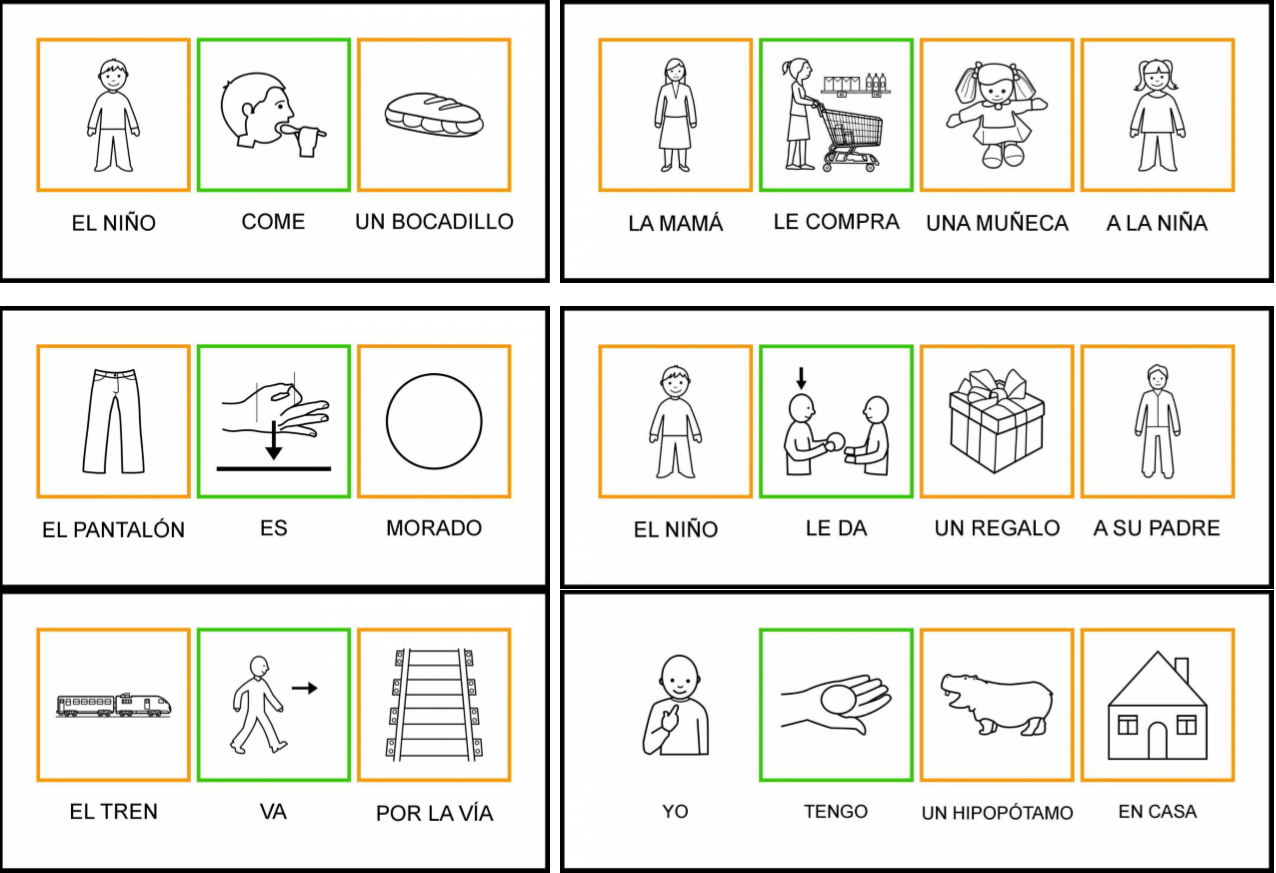
\includegraphics[width=15cm]{Imagenes/Apendice/ApendiceB/apendiceB1}
\end{figure}

\begin{figure}[h]
  \centering
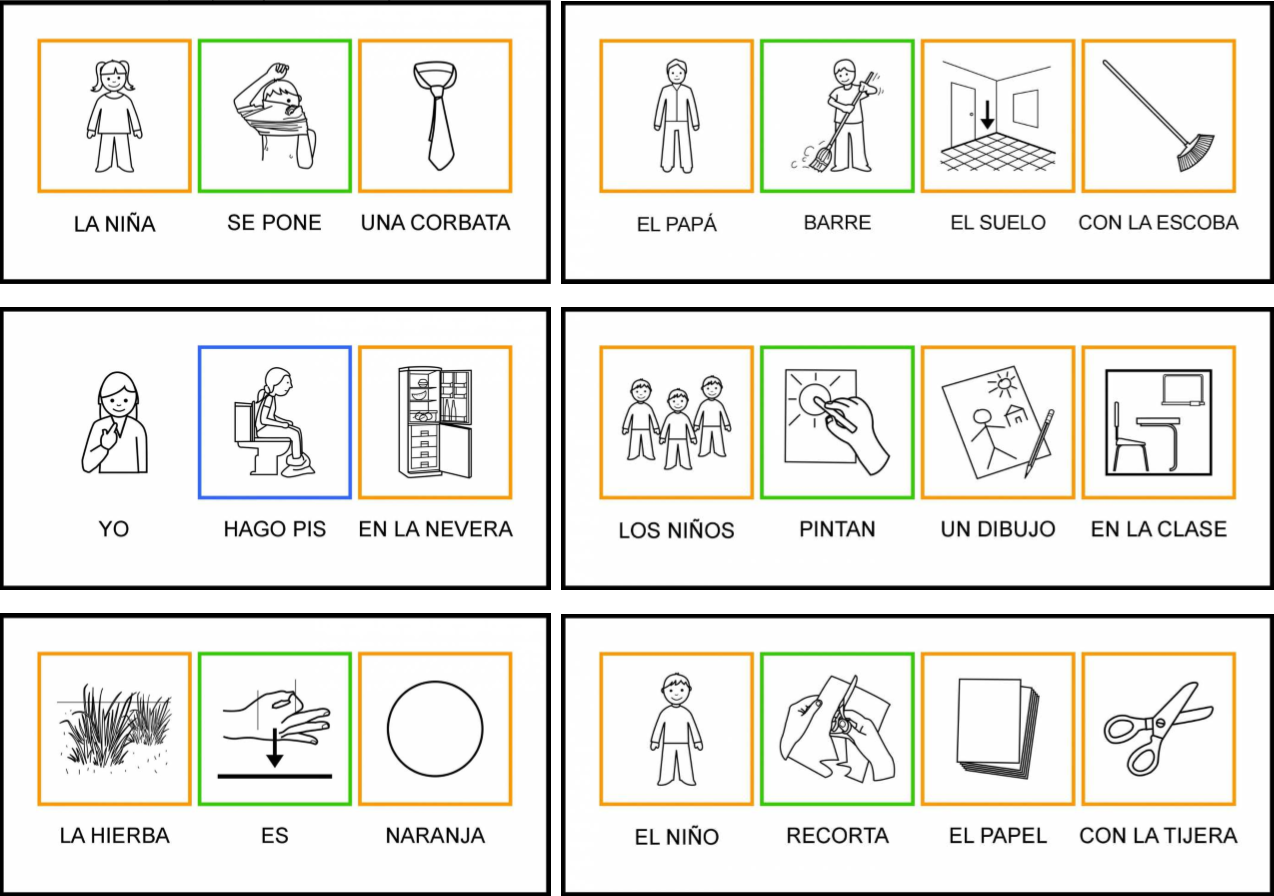
\includegraphics[width=12.2cm]{Imagenes/Apendice/ApendiceB/apendiceB2}
\end{figure}

\begin{figure}[h]
  \centering
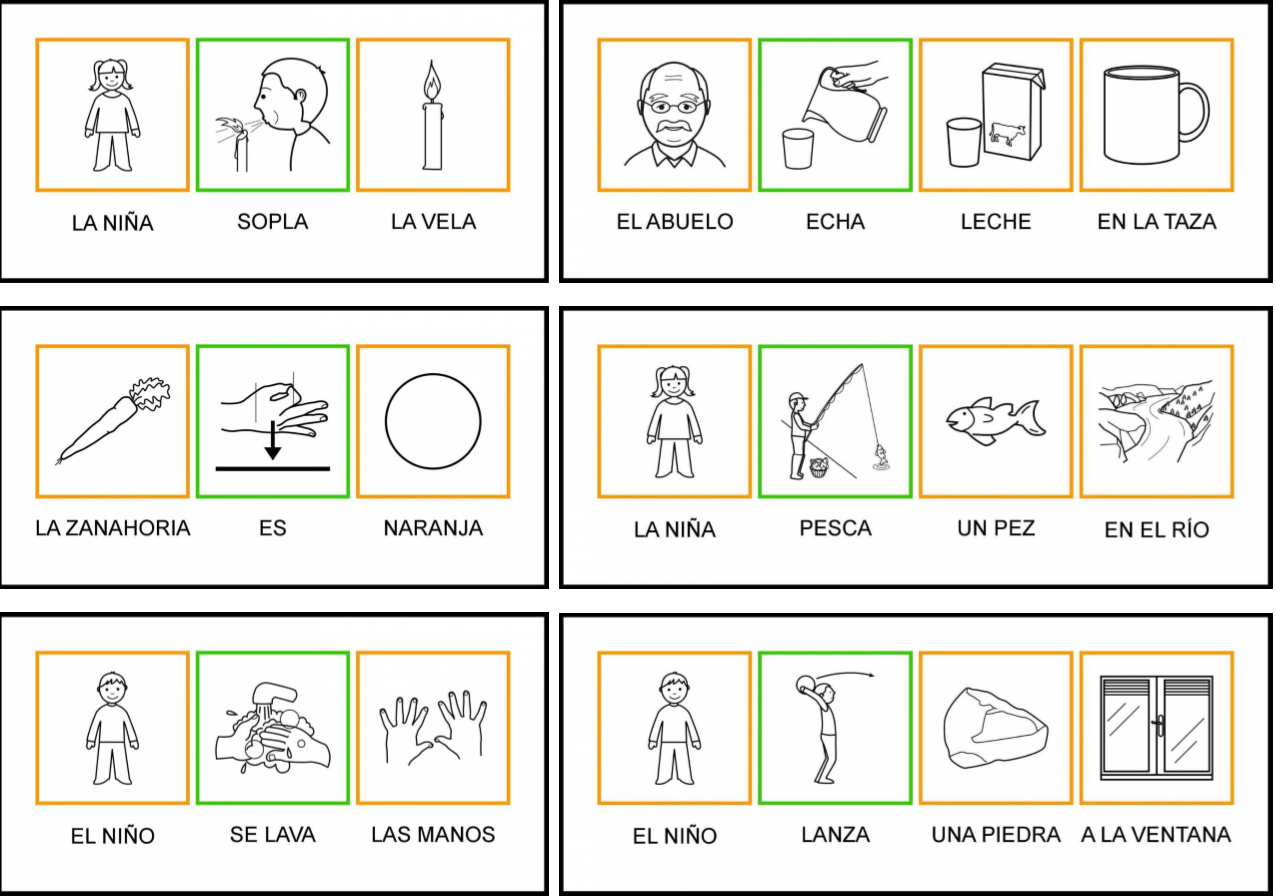
\includegraphics[width=12.2cm]{Imagenes/Apendice/ApendiceB/apendiceB3}
\end{figure}

\begin{figure}[h]
  \centering
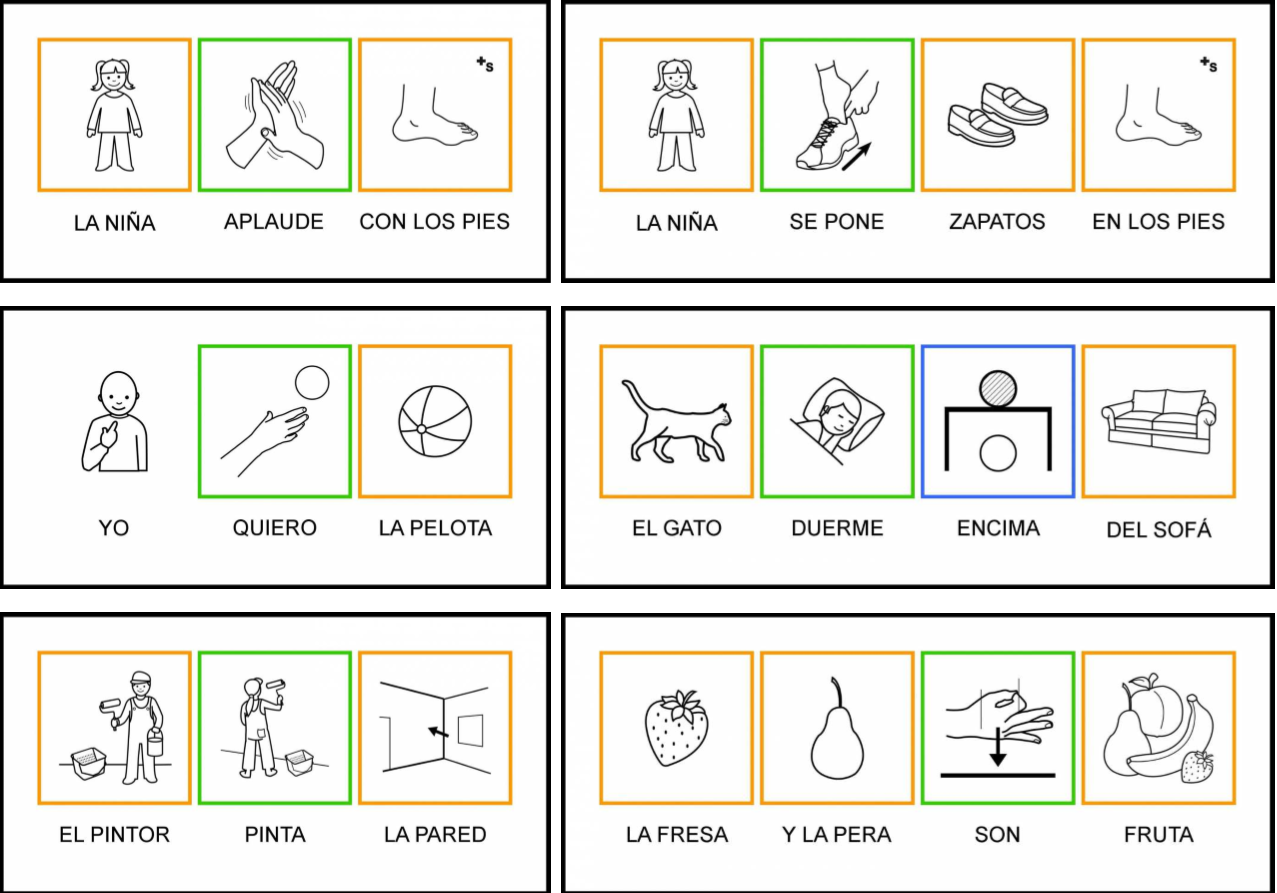
\includegraphics[width=12.2cm]{Imagenes/Apendice/ApendiceB/apendiceB4}
\end{figure}

\begin{figure}[h]
  \centering
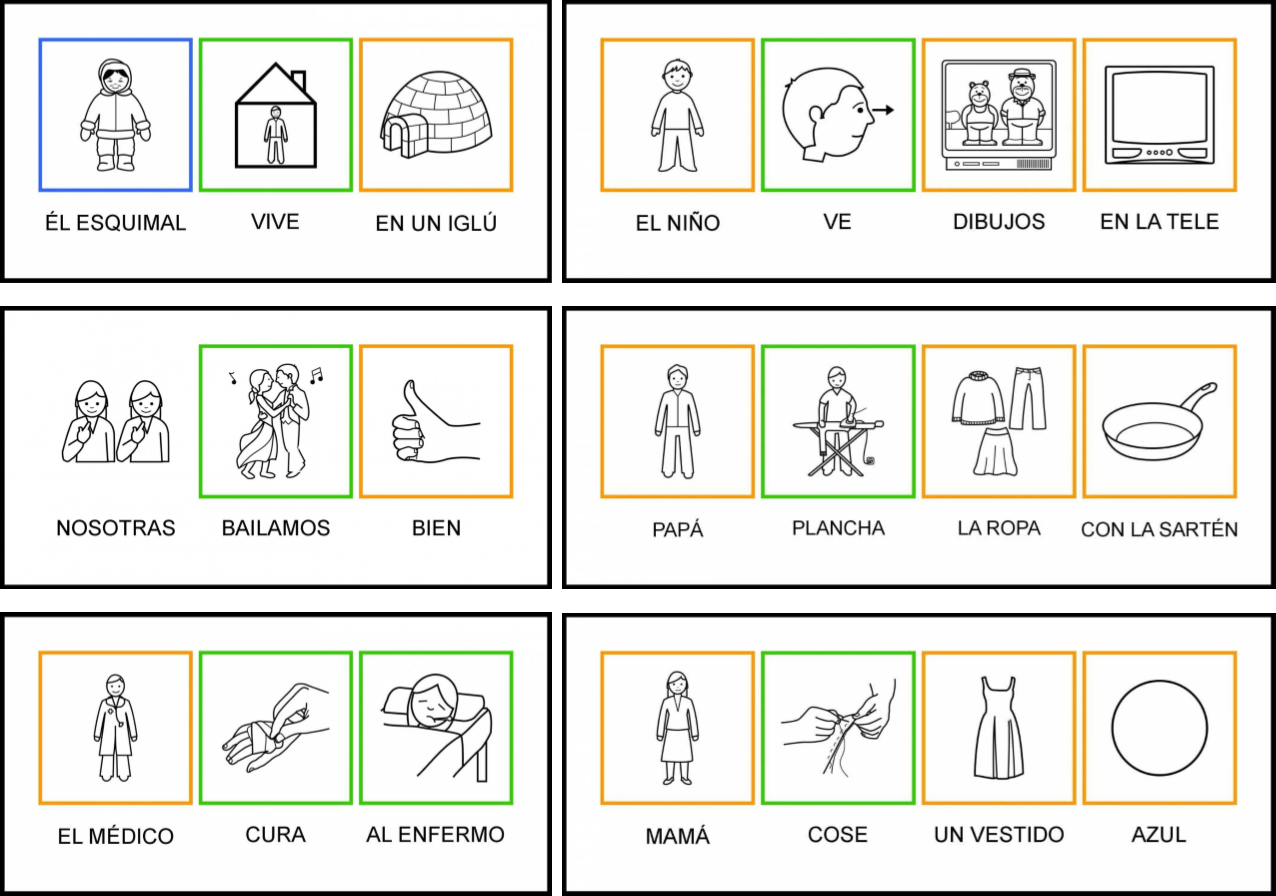
\includegraphics[width=12.2cm]{Imagenes/Apendice/ApendiceB/apendiceB5}
\end{figure}

\begin{figure}[h]
  \centering
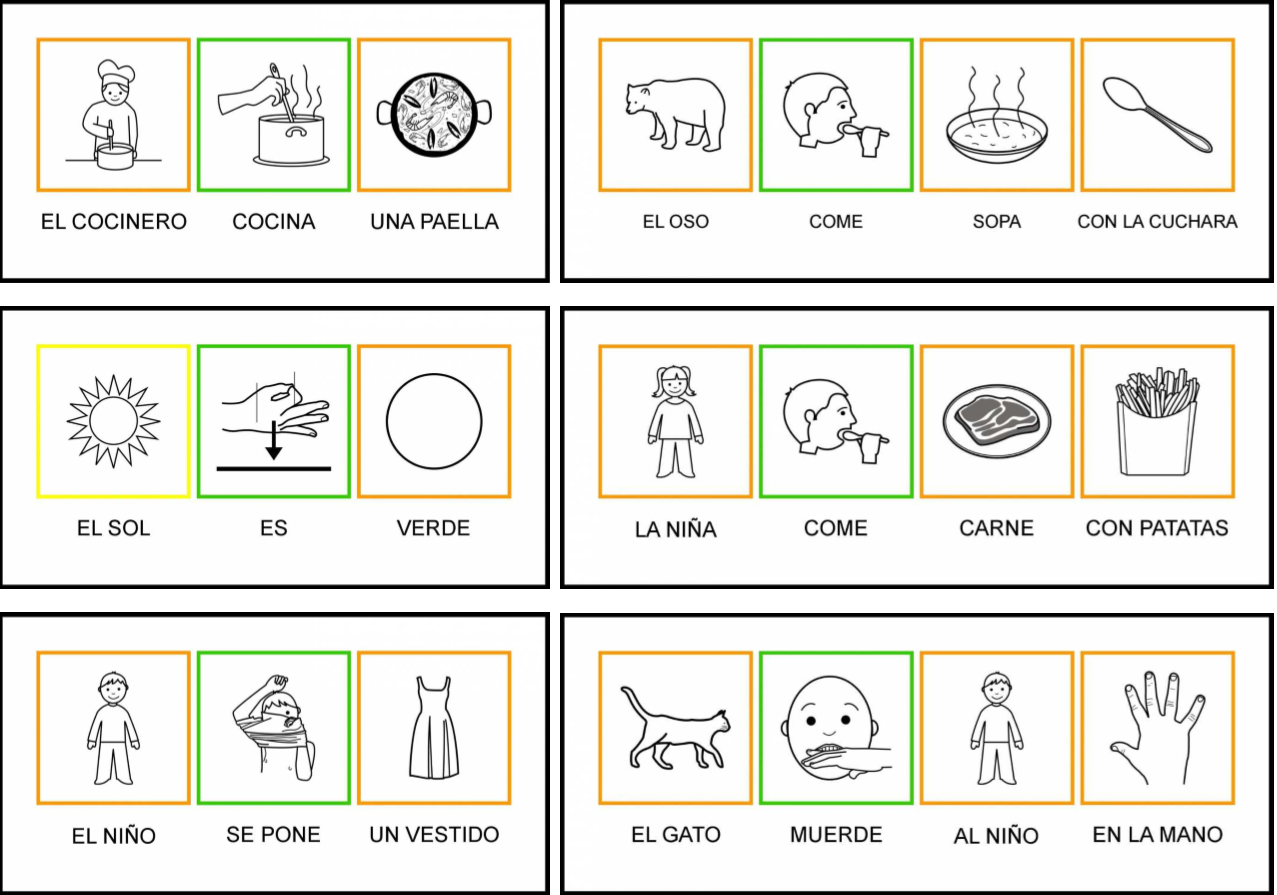
\includegraphics[width=12.2cm]{Imagenes/Apendice/ApendiceB/apendiceB6}
\end{figure}

\begin{figure}[h]
  \centering
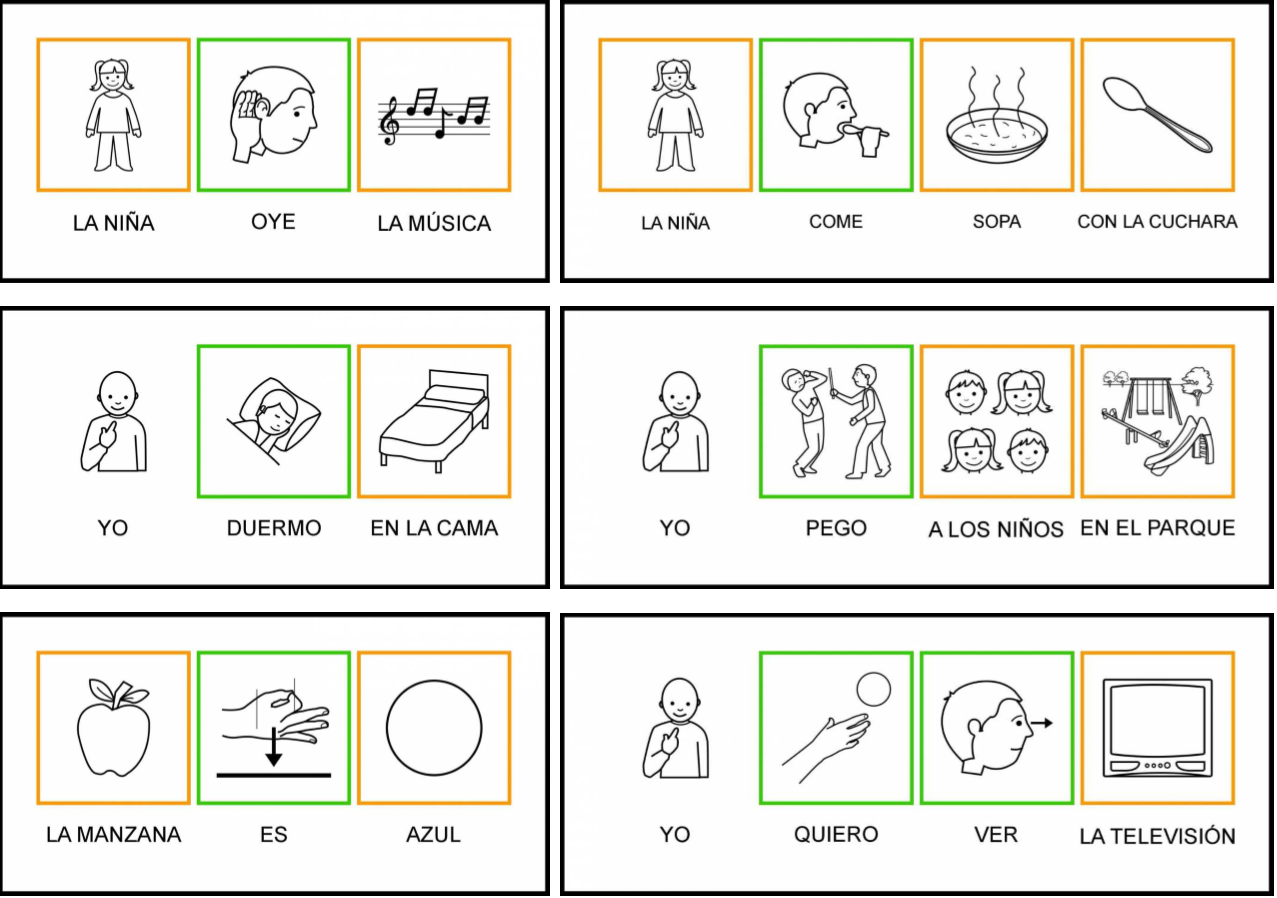
\includegraphics[width=12.2cm]{Imagenes/Apendice/ApendiceB/apendiceB7}
\end{figure}

\begin{figure}[h]
  \centering
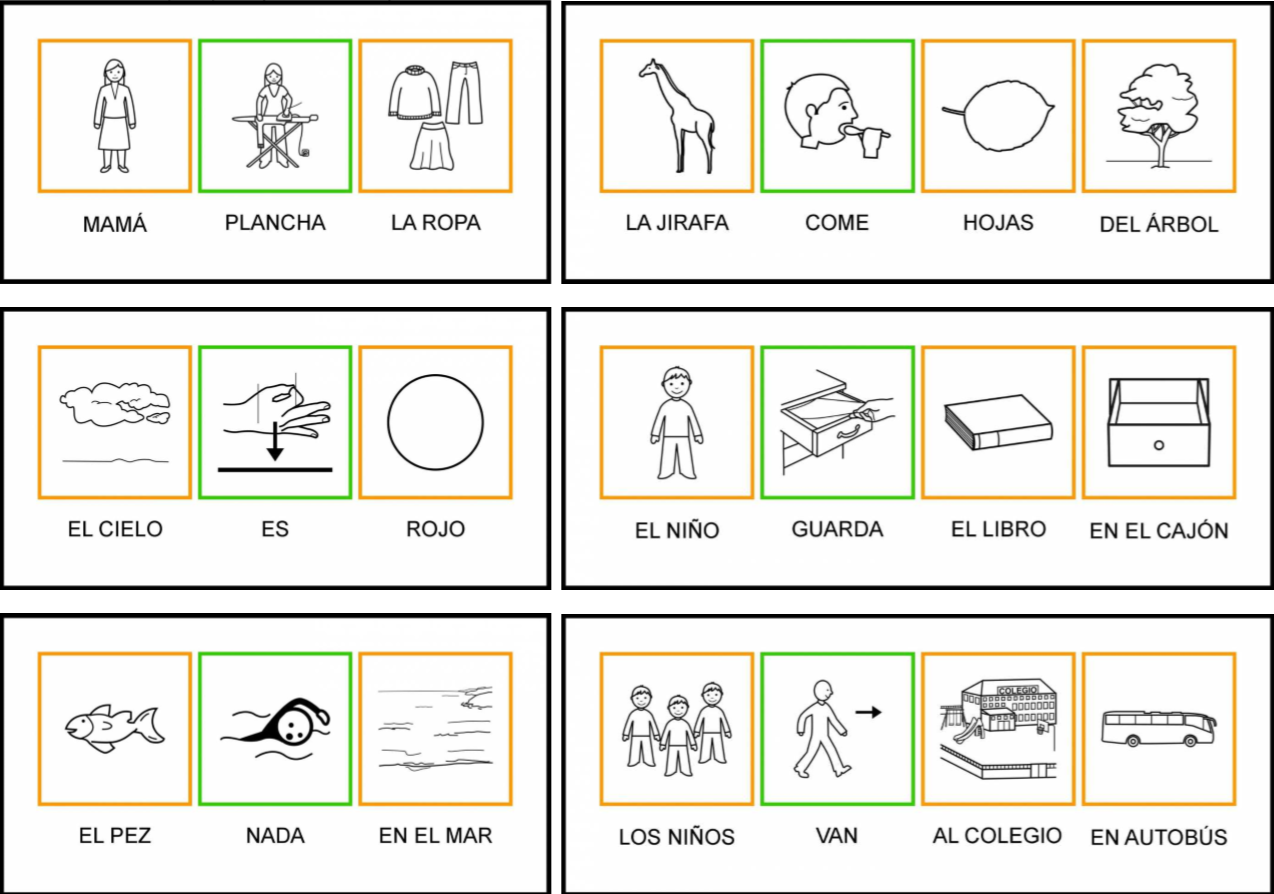
\includegraphics[width=12.2cm]{Imagenes/Apendice/ApendiceB/apendiceB8}
\end{figure}

\begin{figure}[h]
  \centering
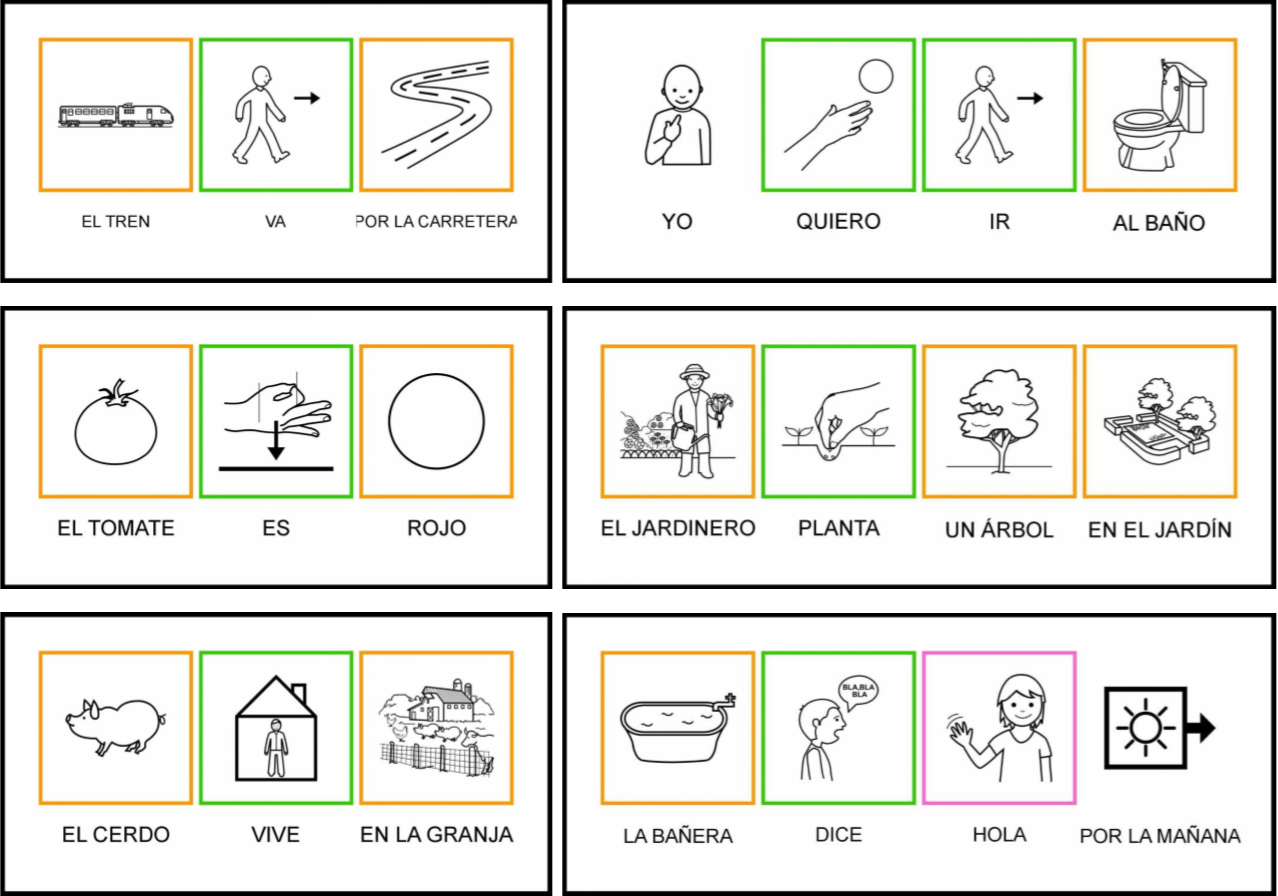
\includegraphics[width=12.2cm]{Imagenes/Apendice/ApendiceB/apendiceB9}
\end{figure}

\begin{figure}[h]
  \centering
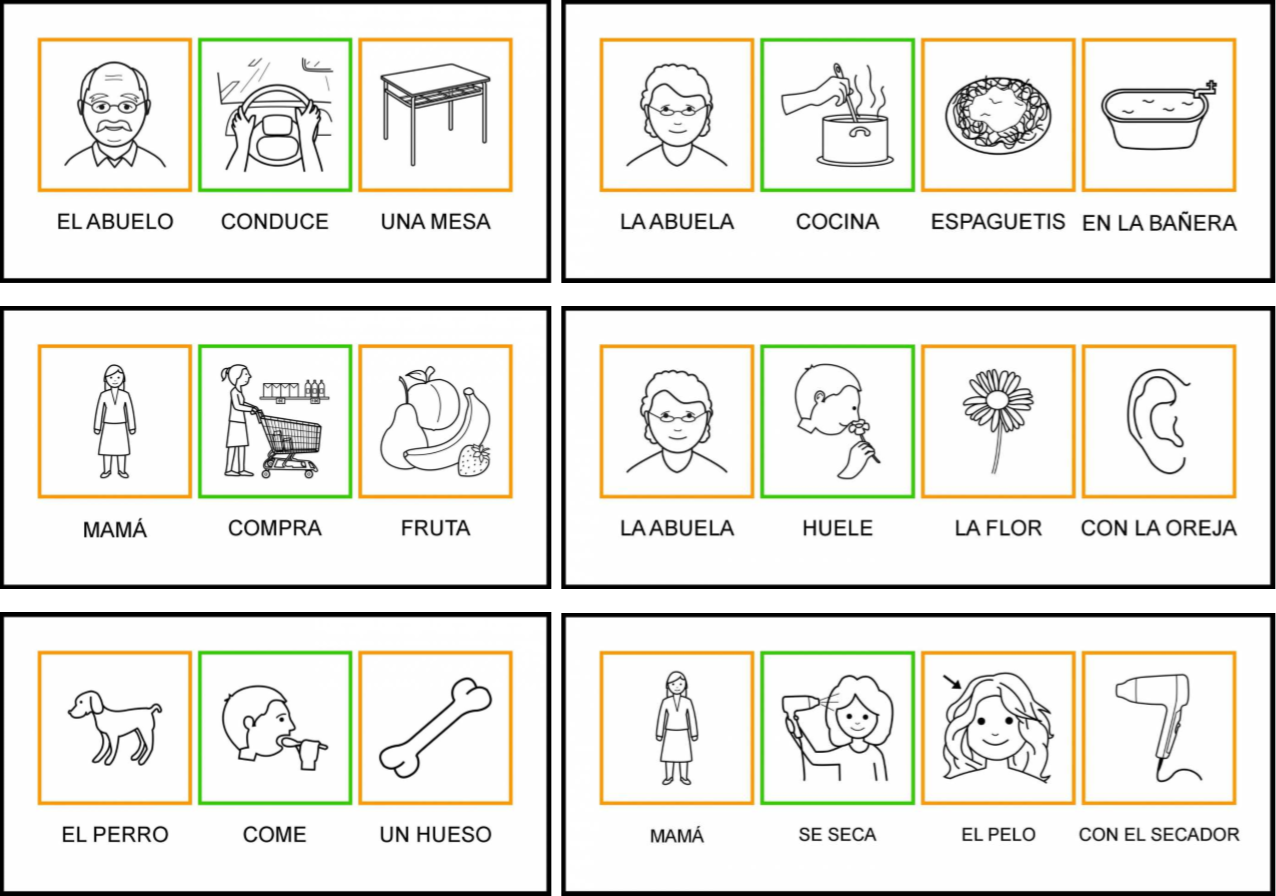
\includegraphics[width=12.2cm]{Imagenes/Apendice/ApendiceB/apendiceB10}
\end{figure}

\begin{figure}[h]
  \centering
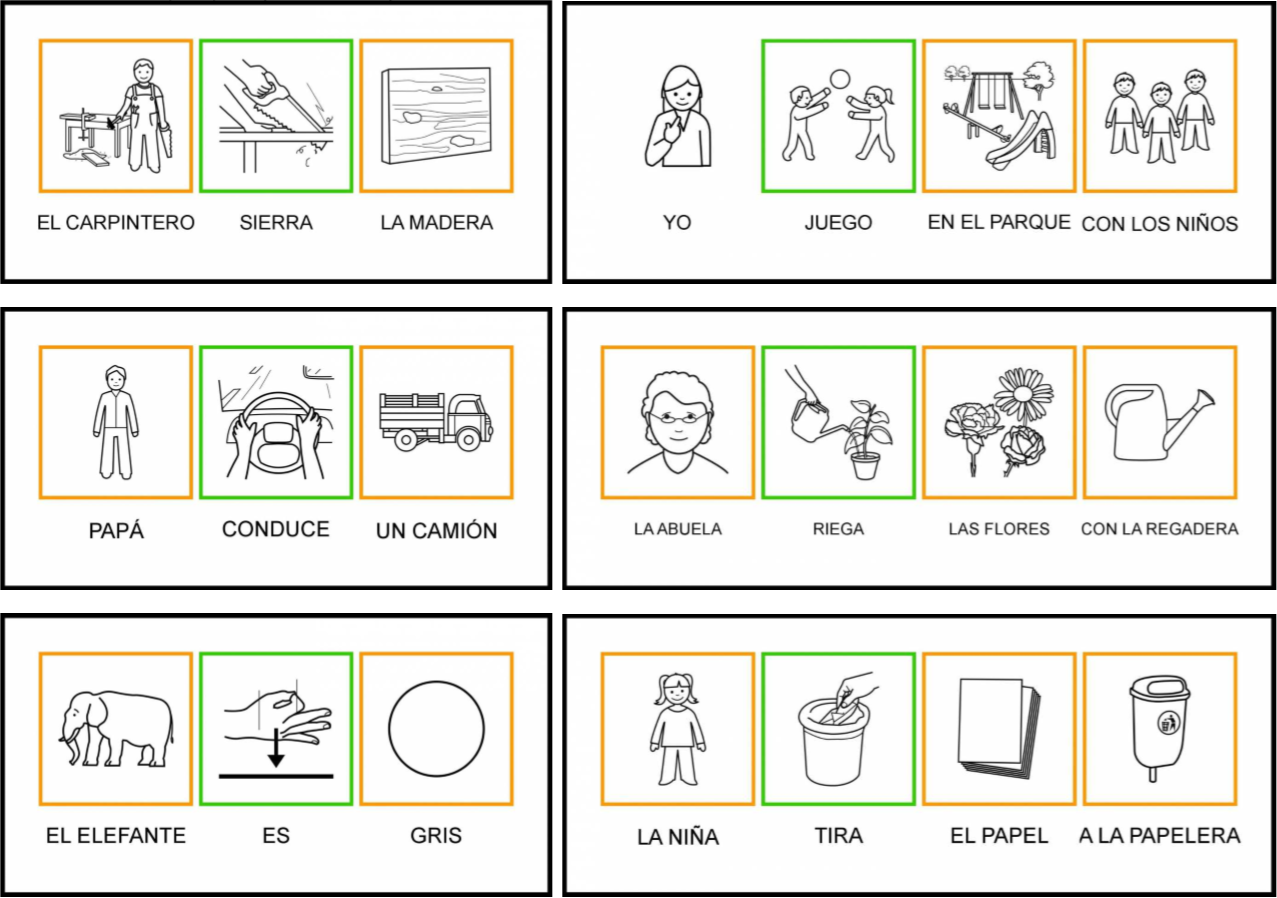
\includegraphics[width=12.2cm]{Imagenes/Apendice/ApendiceB/apendiceB11}
\end{figure}

\begin{figure}[h]
  \centering
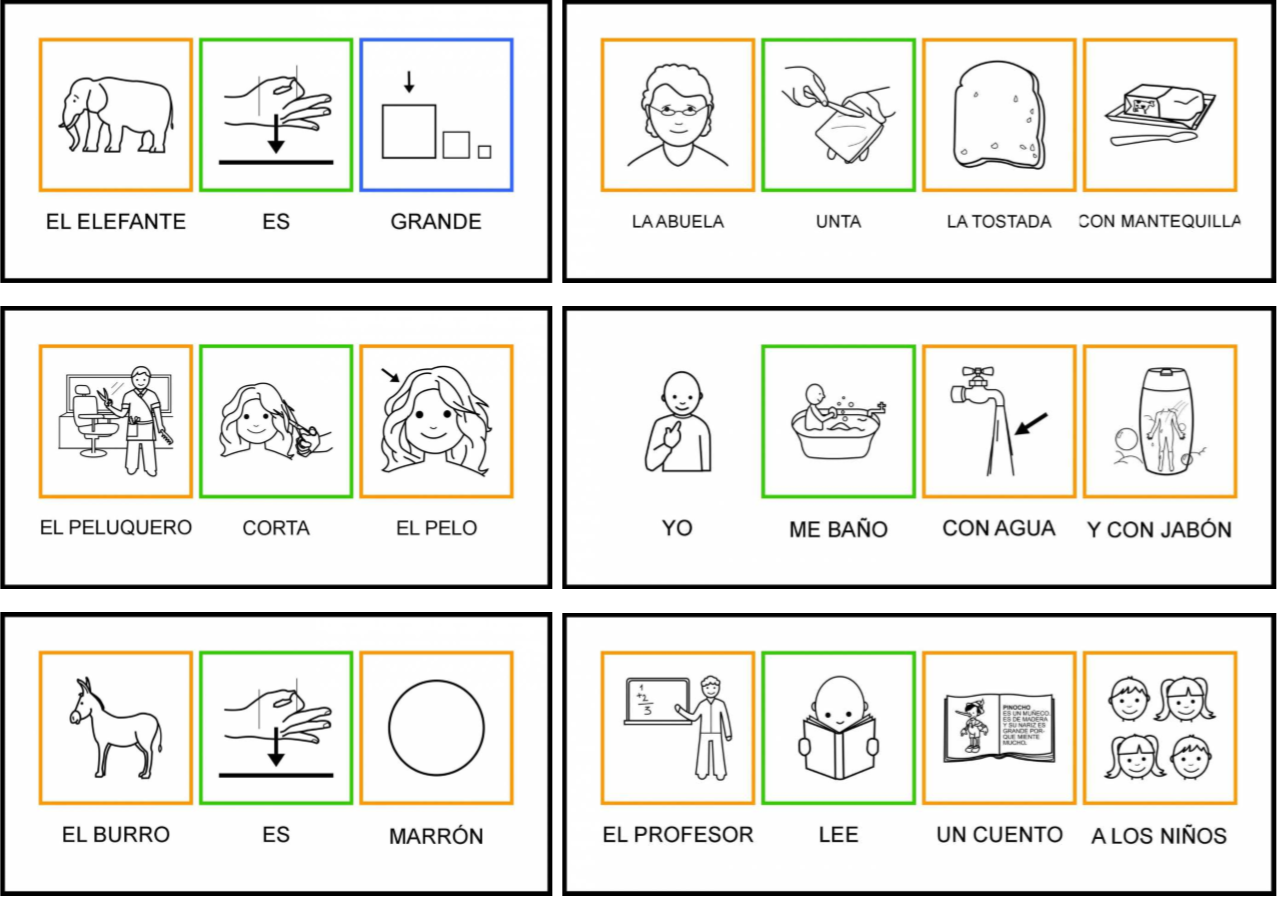
\includegraphics[width=12.2cm]{Imagenes/Apendice/ApendiceB/apendiceB12}
\end{figure}

\begin{figure}[h]
  \centering
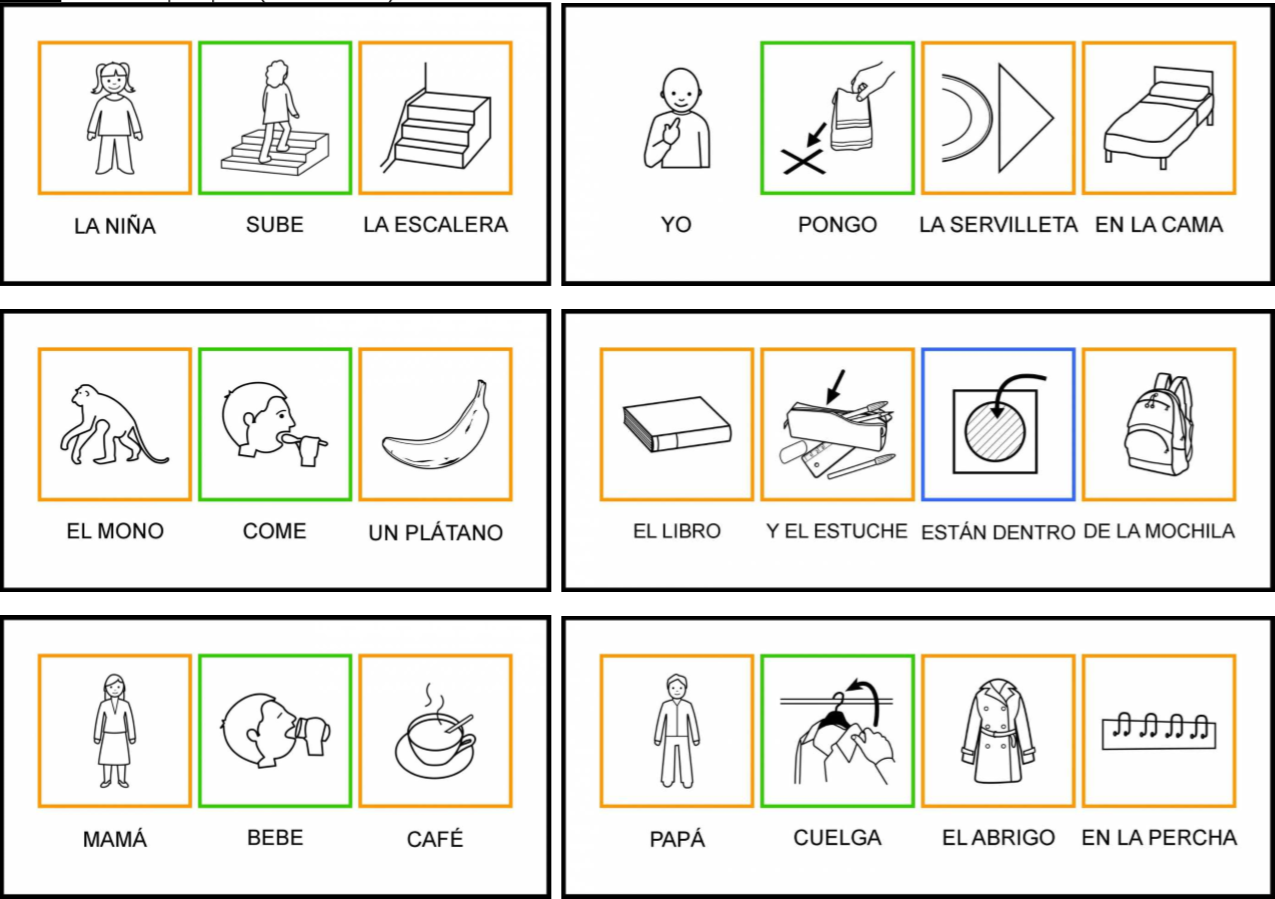
\includegraphics[width=12.2cm]{Imagenes/Apendice/ApendiceB/apendiceB13}
\end{figure}

\begin{figure}[h]
  \centering
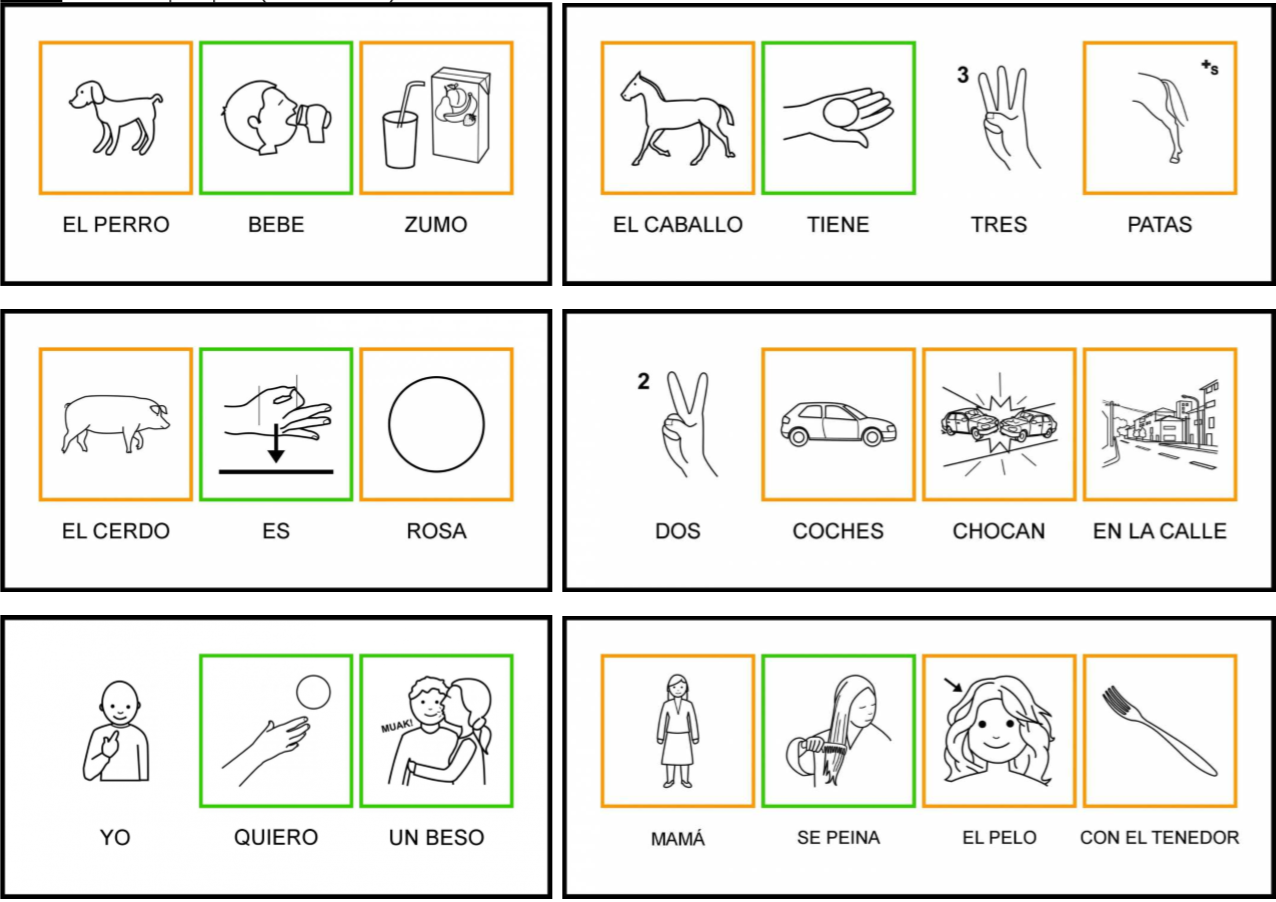
\includegraphics[width=12.2cm]{Imagenes/Apendice/ApendiceB/apendiceB14}
\end{figure}

\begin{figure}[h]
  \centering
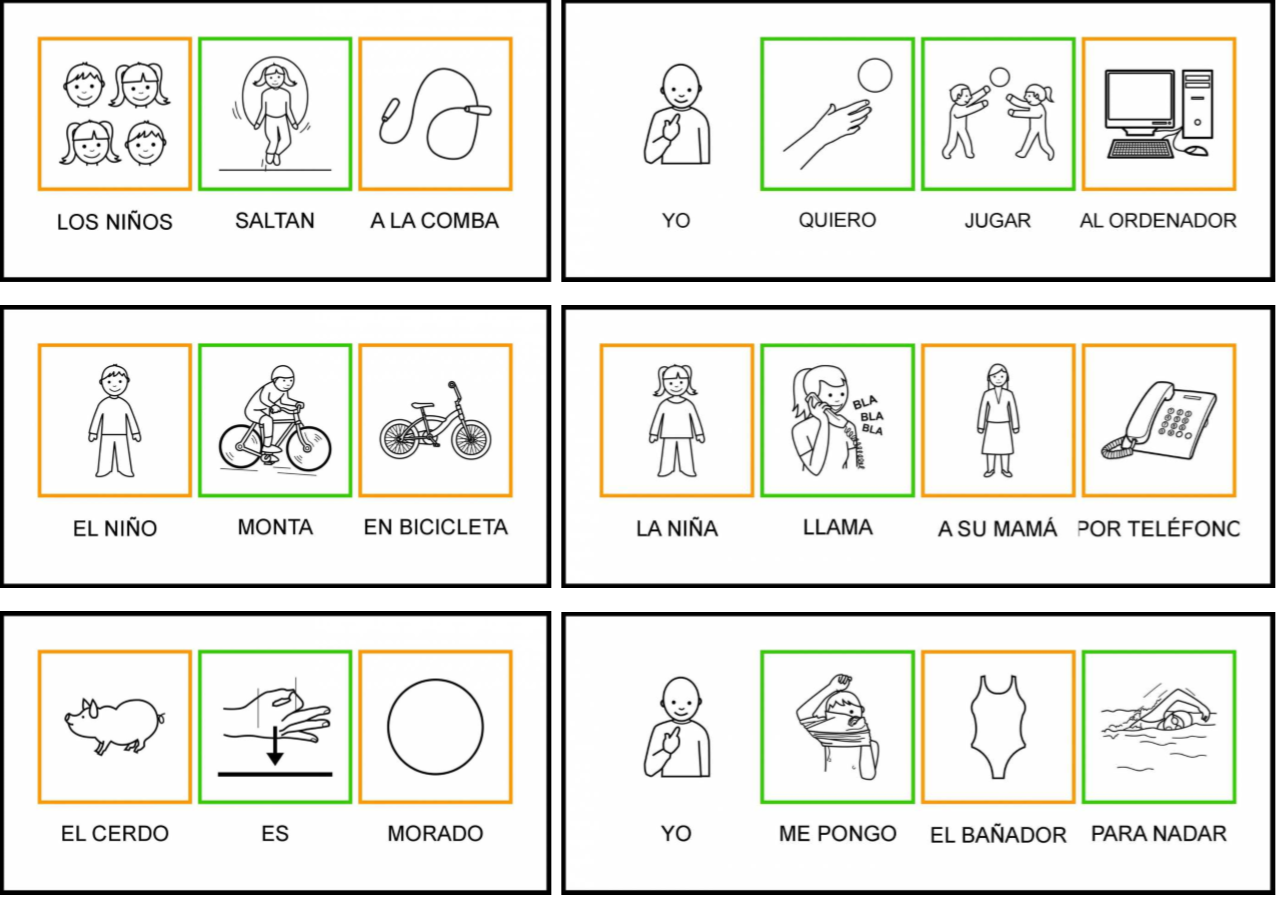
\includegraphics[width=12.2cm]{Imagenes/Apendice/ApendiceB/apendiceB15}
\end{figure}

\begin{figure}[h]
  \centering
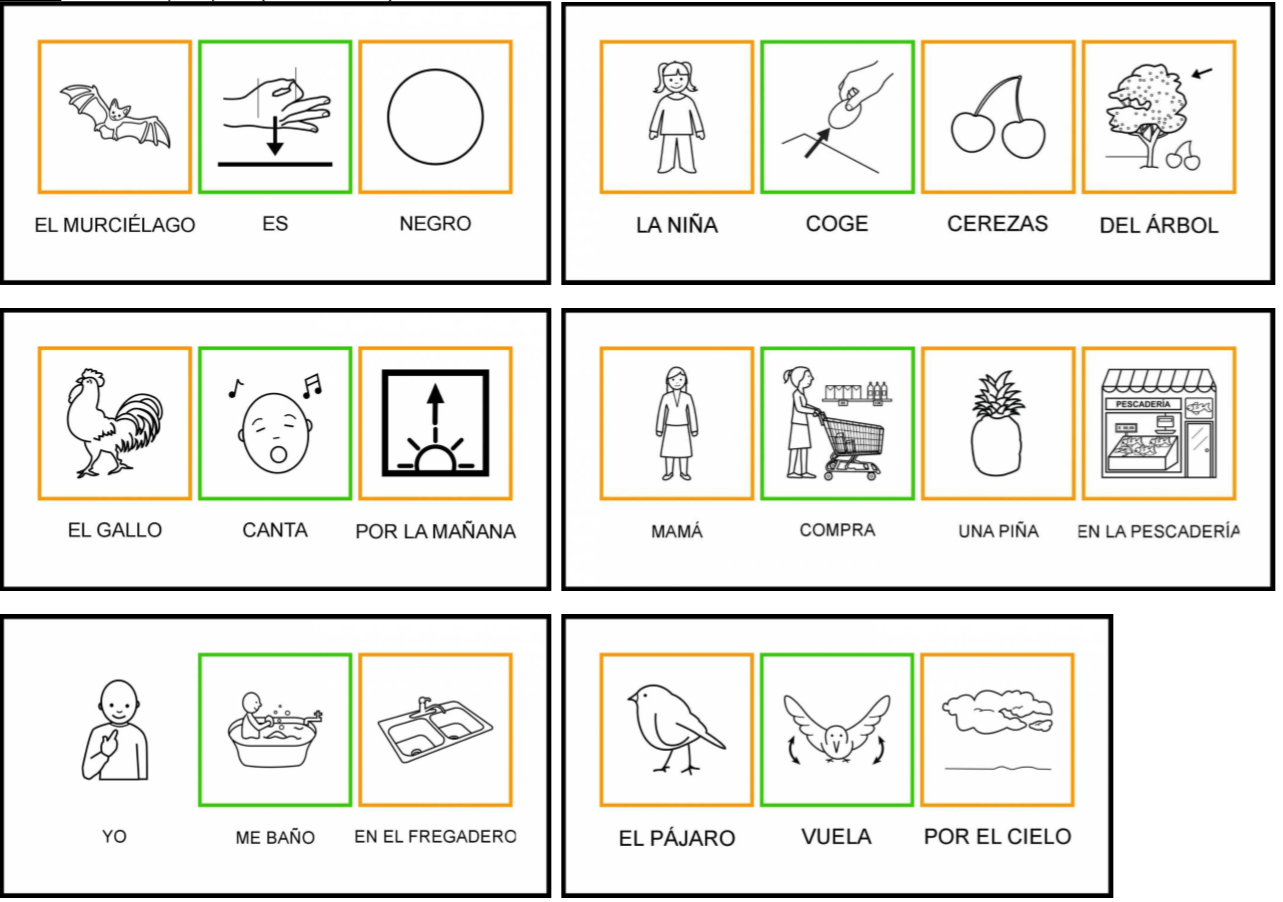
\includegraphics[width=11.4cm]{Imagenes/Apendice/ApendiceB/apendiceB16}
\end{figure}

\begin{figure}[h]
  \centering
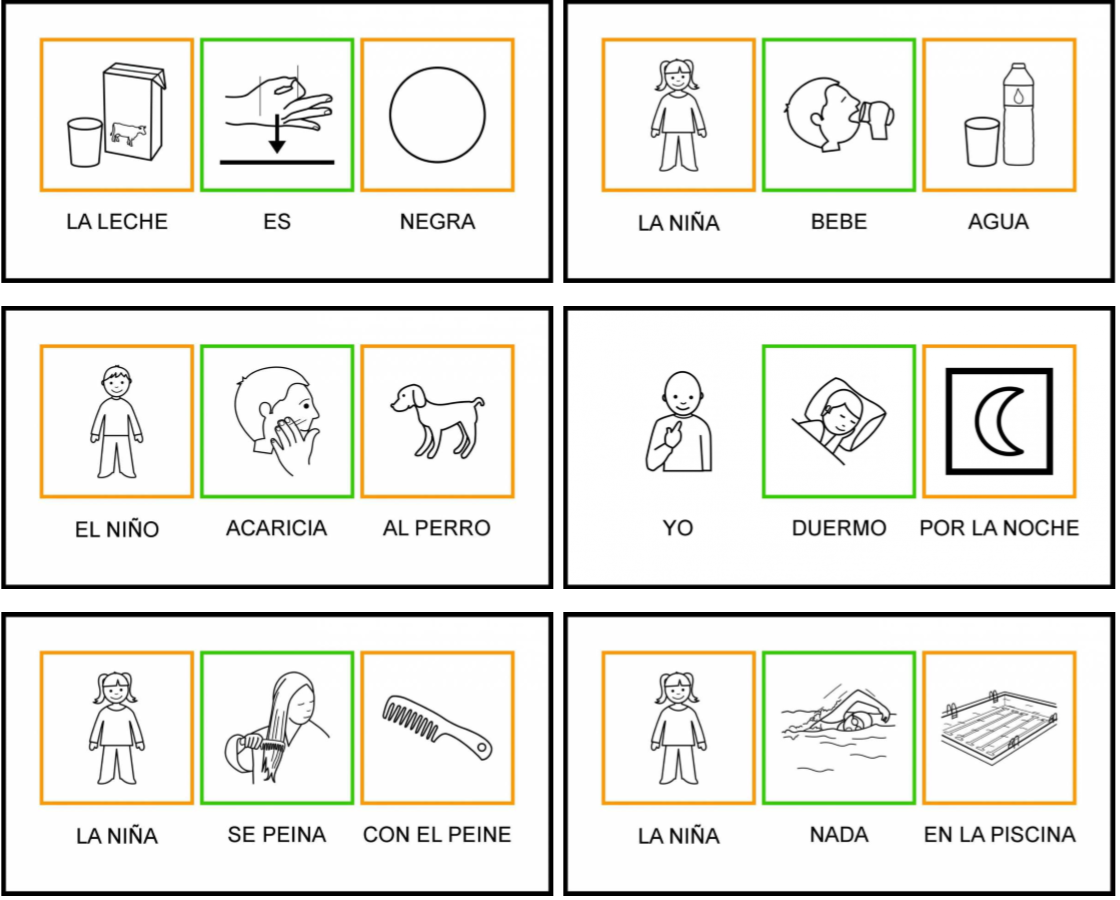
\includegraphics[width=11.3cm]{Imagenes/Apendice/ApendiceB/apendiceB17}
\end{figure}

\begin{figure}[h]
  \centering
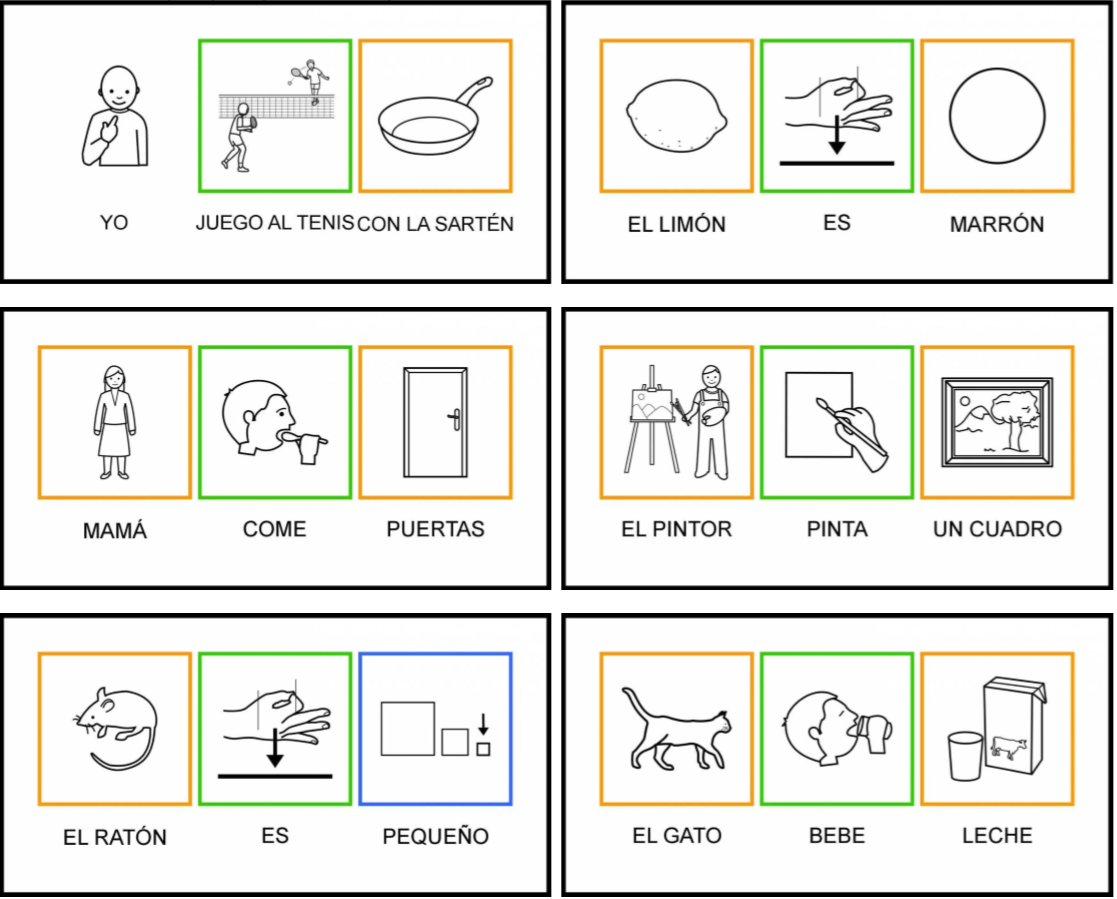
\includegraphics[width=14cm]{Imagenes/Apendice/ApendiceB/apendiceB18}
\end{figure}

\begin{figure}[h]
  \centering
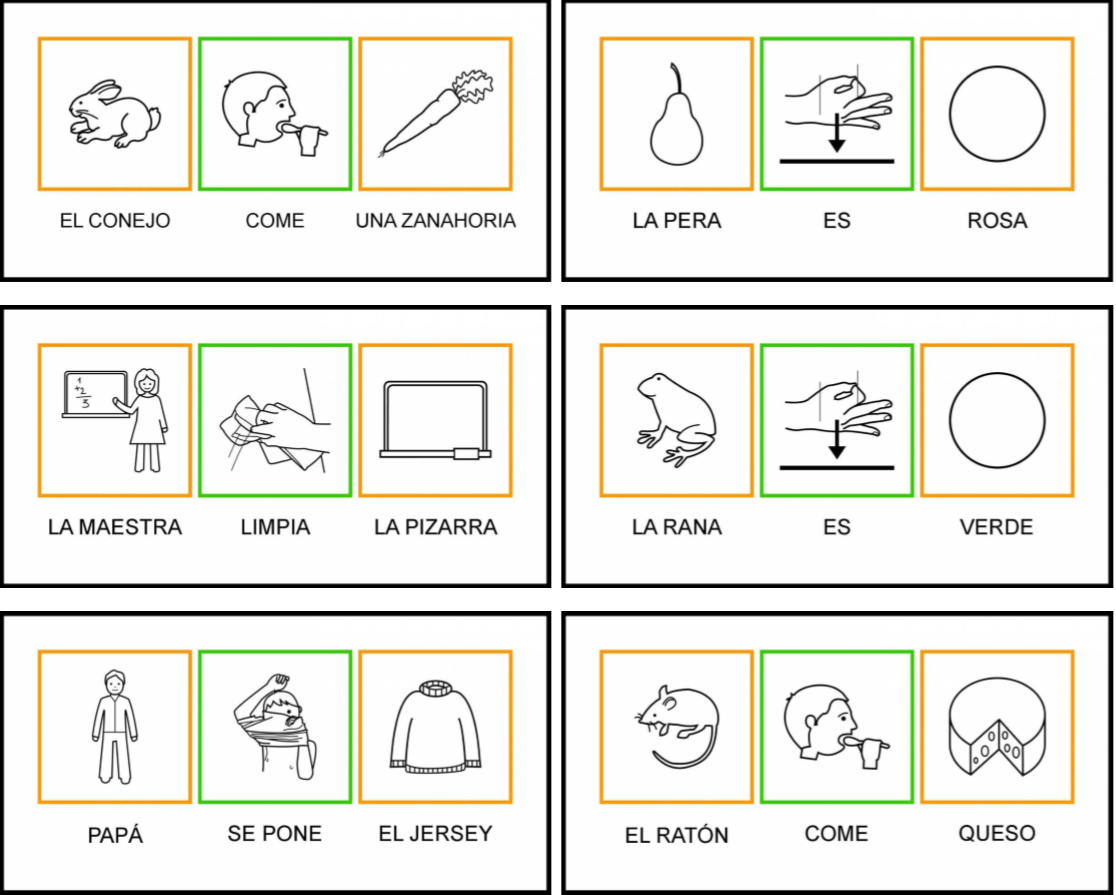
\includegraphics[width=13cm]{Imagenes/Apendice/ApendiceB/apendiceB19}
\end{figure}

\begin{figure}[h]
  \centering
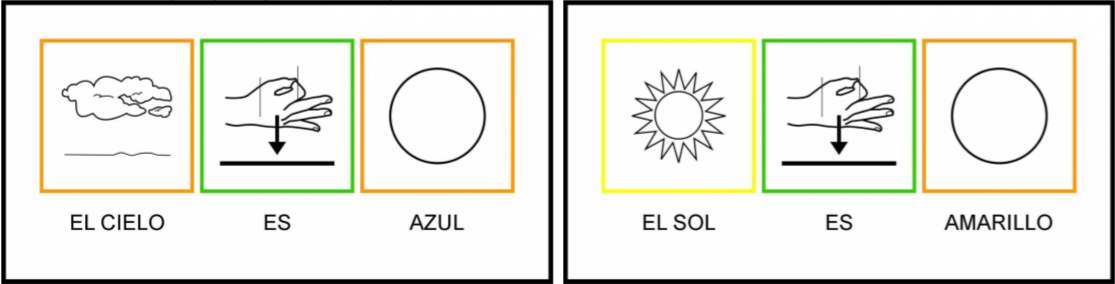
\includegraphics[width=13cm]{Imagenes/Apendice/ApendiceB/apendiceB20}
\end{figure}